% Chapter 4

\chapter{Travaux et apports} % 4th chapter title

\label{Chapter4} % For referencing the chapter elsewhere, use \ref{Chapter4} 


%----------------------------------------------------------------------------------------


\section{Les missions du poste}

\begin{itemize}
    \item L'état de l'art de la partie précédente fait partie des missions.
    \item Modélisation
    \item Simulation
\end{itemize}

Nous souhaitons étudier le comportement mécanique d'un floe après collision avec un autre floe. Les étapes de travail envisagées sont les suivantes:
\begin{enumerate}
    \item Ecire les systèmes differentiels pour les deux floes juste après le choc: pour l' instant on peut considérer que l'un des floes est immobile (celà revient au même si l'on exprimes les vitesses dans un repère lié à ce floe).
    \item On exprime l'EDO vérifiée par les solutions, c'est à dire $q$ pour le premier floes, et $p$ pour le second.
    \item On pourra ensuite simuler ces EDP limites et trouver les valeurs de $p$ et $q$. Autrement dit, on connait la position de chaque point du réseau au temps final.
    \item Si on connait $p$ et/ou $q$, on connait la condition de Dirichlet sur le floe concerné, et on peut ainsi exprimer le déplacement et la possible fracture du floe. 
\end{enumerate}




\section{Présentation des résulats obtenus}



\subsection{Modélisation du contact entre deux floes de glace}

Les floes de glace $\Omega_k$ et $\Omega_l$ sont modélisés par des systèmes masse-ressort (à grande raideur). Pour l'instant, nous considérons une moélisation simplifiée qui assimile un floe à un système de (trois) masses reliés par des ressorts (de constante de raideur $k$), et par des dispositifs visqueux de constante $\mu$.
Nous désignerons par $n+1$ le nombre total de noeuds du floe $\Omega_k$, chaque noeud ayant pour masse $m$. De facon similaire, on définit les constantes $k'$, $\mu'$, $n'+1$, $m'+1$ pour le floe $\Omega_l$. Les positions des noeds de $\Omega_k$ seront noté $(q_i)_{0\leq i\leq n}$, tandis que ceux de $\Omega_l$ seront notés $(p_i)_{0 \leq i\leq n'}$ (voir \cref{fig:contactmanuel}). 

\begin{figure}[!h]
    \centering
    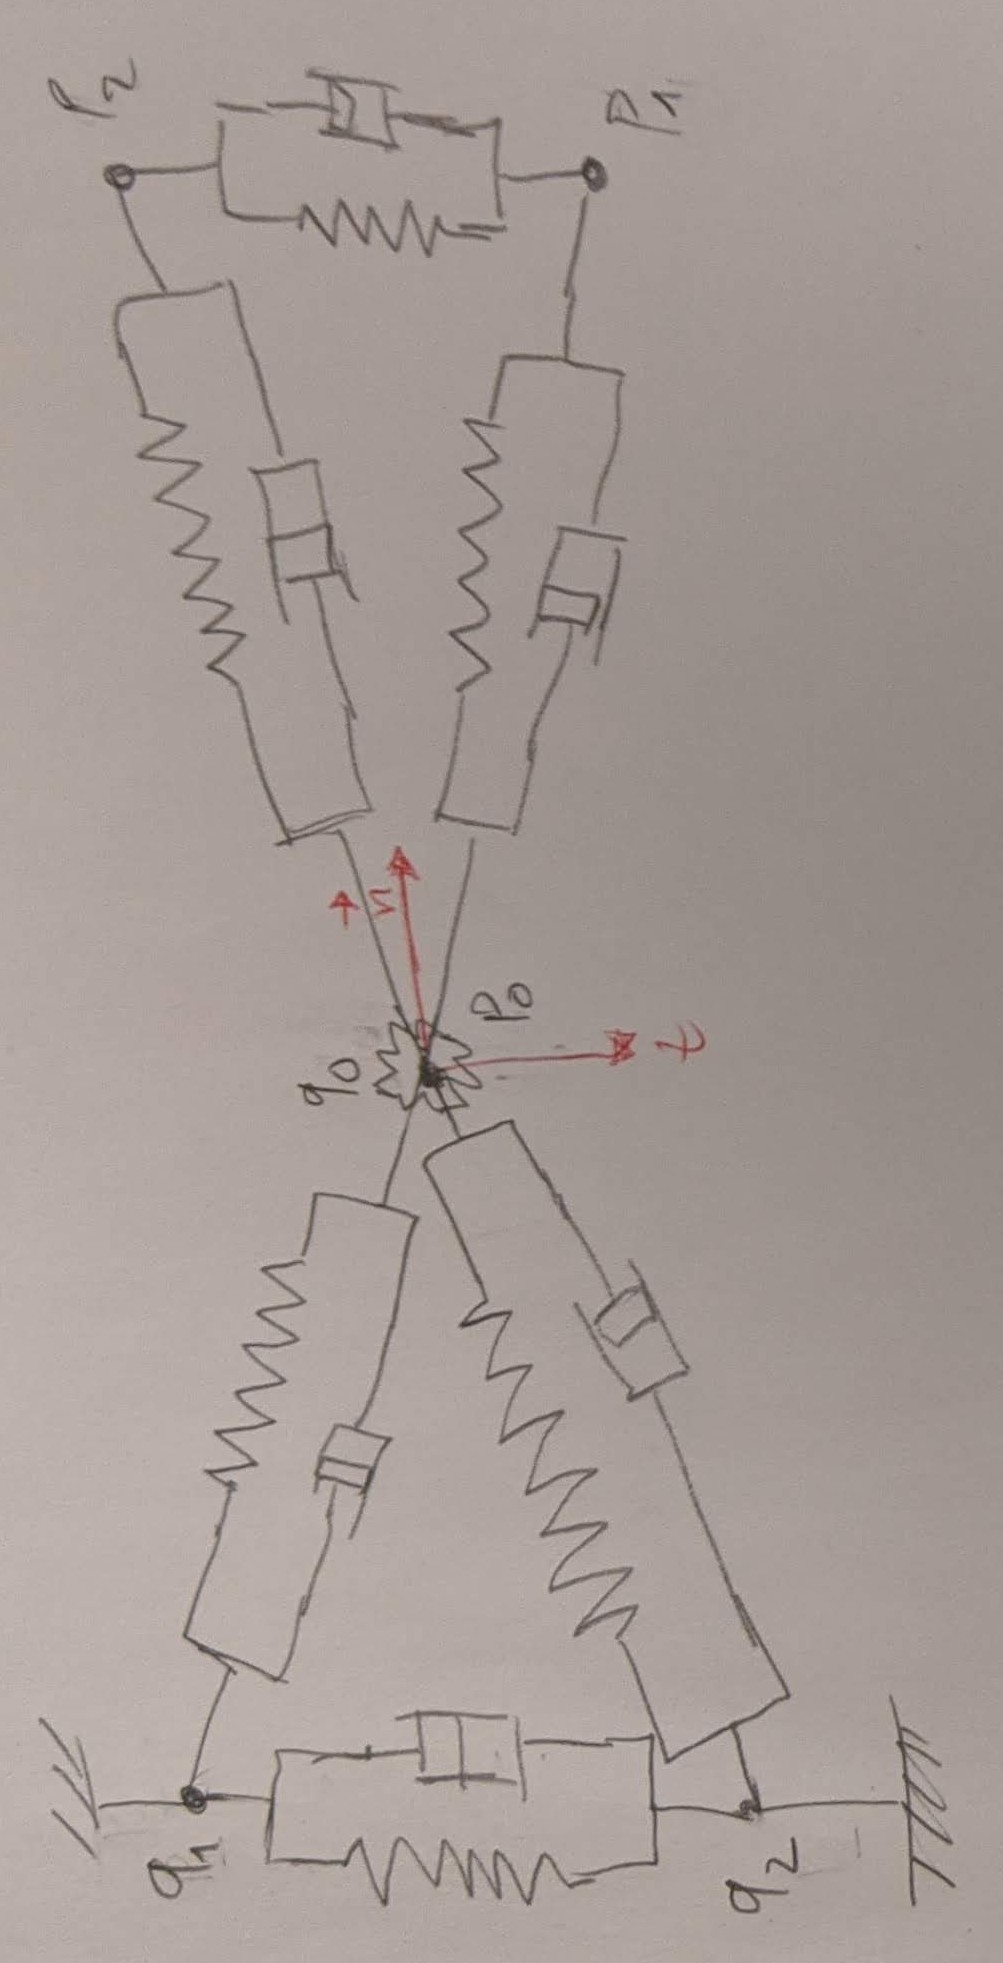
\includegraphics[width=0.3\textwidth, angle=-90]{ContactManuel.jpg}
    \caption{Contact entre deux floes aux points $p_0 = q_0$.}
    \label{fig:contactmanuel}
\end{figure}

\noindent On définit la matrice de contact $C$...(voir these Dimitri), et $L_{0j}$.. et $u_{0j}$ ..

\noindent Comme présenté dans les travaux \parencite[p.186]{balasoiu2020halthesis}, le système différentiel qui modélise la percussion s’écrit comme le couplage de deux sous-systèmes. Le premier, dit système intérieur (SI), est à évolution rapide et modélise la propagation des ondes élastiques dans le système masse-ressort. Ici, nous dérivons facilement et réutilisont le SI comme présenté par \citeauthor{balasoiu2020halthesis}. Le second, dit système extérieur (SE), est à évolution lente et modélise la pénétration de l’objet solide dans le système masse-ressorts. Pour dériver le SE sur le floe $\Omega_k$, nous écrivons l'équation de Newton-Euler linéaire\footnote{La rotation du point matériel $q_0$ n'est pas prise en compte ici, d'où l'abscence de l'équation de Newton-Euler angulaire.} au point de contact $q_0$:
\begin{align}  \label{eq:SE}
m \ddot{\bvec{q}}_0 = \bvec{F}_0 + \bvec{F}^c_0 \,,
\end{align}
où 
\begin{align}  \label{eq:F0}
    \bvec{F}_0 = \sum_{j=0}^{n}C_{0j} \left[  \underbrace{k \left( \Vert \bvec{q}_j - \bvec{q}_0 \Vert - L_{0j} \right) \bvec{u}_{0j}}_{\text{Force de rappel}} - \underbrace{\mu \left\langle \bvec{\dot{q}}_j - \bvec{\dot{q}}_0\,, \bvec{u}_{0j}  \right\rangle  \bvec{u}_{0j}}_{\text{Force de dissipation}}  \right] \,,
\end{align}
représente la somme des forces de reaction et de disssipation exercées par le ressort et le dispositif visqueux sur le noeud $q_0$ ; et $\bvec{F}^c_0(t)$ la force de contact durant la collison entre les deux particules. En supposnat qu'il existe un repère de contact $\mathcal{R}^c = \{ q_0, \bvec{n}, \bvec{t} \}$ associé au floe $\Omega_k$ (voir \cref{fig:contactmanuel}), on peut écrire, pour $(\lambda, \beta) \in \Rdeux$ :
\begin{align}  \label{eq:F0c}
    \bvec{F}_0^c = \lambda \bvec{n} + \beta \bvec{t} \,.
\end{align}
Le système intérieur (SE) s'obtient facilement en combinant les équations \cref{eq:SE,eq:F0,eq:F0c}. Le système intérieur (SI) s'obtient lui (pour les autres noeuds du réseau) en y supprimant la force de contact. On obtient au final:
\begin{align} \tag{$E$} \label{eq:e}
\begin{dcases}
    m \ddot{\bvec{q}}_0 = \bvec{F}_0 + \bvec{F}^c_0  \,, &\qquad \text{(SE)} \\
    m \ddot{\bvec{q}}_i = \bvec{F}_i   \,, \quad \quad \quad \forall 1 \leq i \leq n \,. &\qquad \text{(SI)}
\end{dcases}
\end{align}
En ce qui concerne le floe $\Omega_l$, nous procédons de facons similaire et appliqons la 3ème loi de Newton (action-réaction) pour obtenir le système:
\begin{align} \tag{$E'$} \label{eq:eprime}
\begin{dcases}
    m' \ddot{\bvec{p}}_0 = \bvec{F}^{'}_0 - \bvec{F}^c_0  \,, &\qquad \text{(SE)} \\
    m' \ddot{\bvec{p}}_i = \bvec{F}^{'}_i   \,, \quad \quad \quad \forall 1 \leq i \leq n' \,, &\qquad \text{(SI)}
\end{dcases}
\end{align}
où $(\bvec{F}^{'}_i)_{0 \leq i \leq n'}$ sont définis de facon similaire à $\bvec{F}_0$ (voir \cref{eq:F0}).

Ensuite, il nous faut introduire des conditions portant sur la conservation de l'énergie, et la condition de non-interpénétration de Signorini\dots



\subsubsection*{Modélisation et simulation 1D}

Nous effectuons ici une modélisation 1D complète. Un floe est modélisé par un système masse-ressort de deux noeuds.
Le floe 1 est immobilisé face au mur, et le floe 2 approche à la vitesse $\bvec{v}_0$. On identifie les noeuds $q_0$
et $p_0$ de la section précédente à leur masses respectives $m$ et $m'$ (voir \ref{fig:contact1d}).
\begin{figure}[!h]
    \centering
    \frame{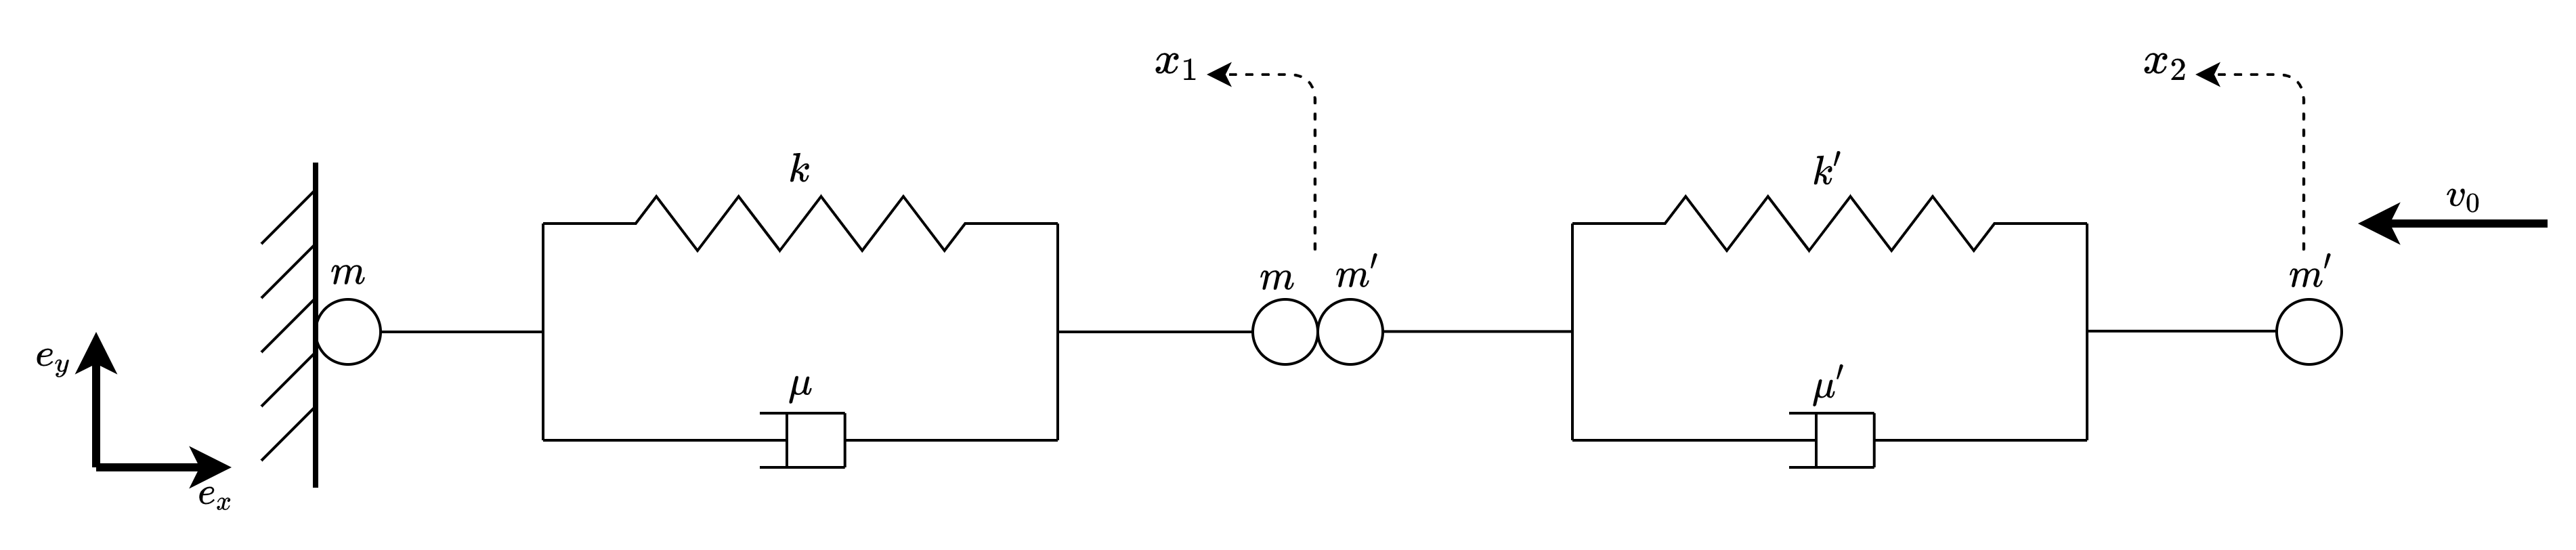
\includegraphics[width=0.8\textwidth]{Percussion1D-Systeme}}
    \caption{Contact 1D entre deux floes.}
    \label{fig:contact1d}
\end{figure}

\noindent On suppose que durant la dynamique non régulière, les masses $m$ et $m'$ en contact forment une seule masse
$m+m'$ dont
le déplacement des donné par la variable $x_1(t)$. Le déplacement de la masse $m'$ à l'autre bout du système est nommé
$x_2(t)$. La masse $m$ fixée au mur ne sera pas étudiée ici. Nous faisons à présent le bilan des forces qui
s'exercent ces
deux masses.
\begin{figure}[!h]
     \begin{subfigure}[b]{0.4\textwidth}
         \centering
         \frame{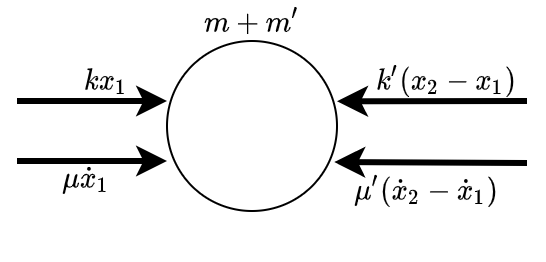
\includegraphics[width=\textwidth]{Percussion1D-Masse1}}
         \caption{Sur $m+m'$.}
         \label{fig:bilan1}
     \end{subfigure}
%     \hfill
     \begin{subfigure}[b]{0.3\textwidth}
         \centering
         \frame{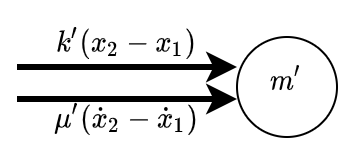
\includegraphics[width=\textwidth]{Percussion1D-Masse2}}
         \caption{Sur $m'$.}
         \label{fig:bilan2}
     \end{subfigure}
        \caption{Bilan des forces appliquée sur les noeuds du système.}
        \label{fig:bilan}
\end{figure}

En orientant convenablement le système (voir \cref{fig:contact1d}), on applique les lois de Newton-Euler linéaires
pour obtenir les système suivant et ses conditions initiales \footnote{J'ai des doutes sur cette condition
initiale. La  vitesse initiale de $x_1$ est-elle vraiment $0$?}:
\begin{align}
    \begin{dcases}
    (m+m')\ddot x_1 = kx_1 + \mu \dot x_1 - k'(x_2 - x_1) - \mu'(\dot x_2 - \dot x_1) \\
        m' \ddot x_2 =  k'(x_2 - x_1) + \mu'(\dot x_2 - \dot x_1) \\
    \end{dcases}
\end{align}
À l'instant initial $t_0$, on a le système suivant
\begin{align} \label{eq:percussion1d}
    \begin{dcases}
    (x_1(t_0), x_2(t_0)) = (0,0) \\
    (\dot x_1(t_0), \dot x_2(t_0)) = (0,v_0)
    \end{dcases}
\end{align}
En posant $X = (x_1, x_2)^T \in \mathbb{R}^2$, l' \cref{eq:percussion1d} devient
\begin{align}
    \underbrace{\mymat{m+m'}{0}{0}{m'}}_{A} \myvec{\ddot{x}_1}{\ddot{x}_2} = \underbrace{\mymat{\mu +
    \mu^\prime}{-\mu'}{-\mu'}{\mu'}}_{B}
    \myvec{\dot{x}_1}{\dot{x}_2} + \underbrace{\mymat{k+k'}{-k'}{-k'}{k'}}_{C} \myvec{x_1}{x_2} \,.
\end{align}
Puisque $m, m'\neq 0$, la matrice $A$ est inversible et on obtient au final le problème de Cauchy suivant:

\begin{align} \label{eq:percussion1d2}
    \begin{dcases}
        \ddot{X}(t) = B' \dot{X}(t) + C'X(t) \,, \\
        (X(t_0), \dot X (t_0)) = \left( \myvec{0}{0}, \myvec{0}{v_0} \right) \,,
    \end{dcases}
\end{align}
avec $B' = A^{-1}B$ et $C' = A^{-1}C$.

\noindent Il s'agit la d'un suytème d'EDO du deuxième ordre à coefficients constants. Transformons le en un système du
premier ordre pour
une
résolusiotn plus aisée. On pose donc $Y= (X, \dot X)^T = (x_1, x_2, \dot{x}_1, \dot{x}_2)^T \in \mathbb{R}^4$ et le
système
\ref{eq:percussion1d2}
devient
\begin{align}
    \begin{dcases}
        \dot{Y}(t)= E Y(t) \\
        Y(t_0) = (0,0,0,v_0)^T
    \end{dcases}
\end{align}
avec la matrice par blocs \[ E = \mymat{0}{I_2}{C'}{B'} \,, \] où $I_2$ désigne la matrice identité de
$\mathbb{R}^{2\times2}$.






\section{Les apports du stage}

%\begin{itemize}
%    \item L' utilisation de TIKZ
%\end{itemize}